% AER E 361 Mission Report Template
% Spring 2023
% Template created by Yiqi Liang and Professor Matthew Nelson

% Document Configuration DO NOT CHANGE
\documentclass[12 pt]{article}
% --------------------LaTeX Packages---------------------------------
% The following are packages that are used in this report.
% DO NOT CHANGE ANY OF THE FOLLOWING OR YOUR REPORT WILL NOT COMPILE
% -------------------------------------------------------------------

\usepackage{hyperref}
\usepackage{parskip}
\usepackage{titlesec}
\usepackage{titling}
\usepackage{graphicx}
\usepackage{graphviz}
\usepackage[T1]{fontenc}
\usepackage{titlesec, blindtext, color} %for LessIsMore style
\usepackage{tcolorbox} %for references box
\usepackage[hmargin=1in,vmargin=1in]{geometry} % use 1 inch margins
\usepackage{float}
\usepackage{tikz}
\usepackage{svg} % Allows for SVG Vector graphics
\usepackage{textcomp, gensymb} %for degree symbol
\hypersetup{
	colorlinks=true,
	linkcolor=blue,
	urlcolor=cyan,
}
\usepackage{biblatex}
\addbibresource{lab-report-bib.bib}
\usepackage{amsmath}
\usepackage{listings}
\usepackage{multicol}
\usepackage{array}

\usepackage{hologo} %KYR: for \BibTeX
%\usepackage{algpseudocode}
%\usepackage{algorithm}
% This configures items for code listings in the document
\usepackage{xcolor}

\usepackage{fancyhdr} % Headers/Footers
\usepackage{siunitx} % SI units
\usepackage{csquotes} % Display Quote
\usepackage{microtype} % Better line breaks

\definecolor{commentsColor}{rgb}{0.497495, 0.497587, 0.497464}
\definecolor{keywordsColor}{rgb}{0.000000, 0.000000, 0.635294}
\definecolor{stringColor}{rgb}{0.558215, 0.000000, 0.135316}
\definecolor{mygreen}{rgb}{0,0.6,0}
\definecolor{mygray}{rgb}{0.5,0.5,0.5}
\definecolor{mymauve}{rgb}{0.58,0,0.82}

\lstdefinestyle{customc}{
  belowcaptionskip=1\baselineskip,
  breaklines=true,
  frame=L,
  xleftmargin=\parindent,
  language=C,
  showstringspaces=false,
  basicstyle=\footnotesize\ttfamily,
  keywordstyle=\bfseries\color{green!40!black},
  commentstyle=\itshape\color{purple!40!black},
  identifierstyle=\color{blue},
  stringstyle=\color{orange},
 }

 \lstset{ %
  backgroundcolor=\color{white},   % choose the background color; you must add \usepackage{color} or \usepackage{xcolor}
  basicstyle=\footnotesize,        % the size of the fonts that are used for the code
  breakatwhitespace=false,         % sets if automatic breaks should only happen at whitespace
  breaklines=true,                 % sets automatic line breaking
  captionpos=b,                    % sets the caption-position to bottom
  commentstyle=\color{commentsColor}\textit,    % comment style
  deletekeywords={...},            % if you want to delete keywords from the given language
  escapeinside={\%*}{*)},          % if you want to add LaTeX within your code
  extendedchars=true,              % lets you use non-ASCII characters; for 8-bits encodings only, does not work with UTF-8
  frame=tb,	                   	   % adds a frame around the code
  keepspaces=true,                 % keeps spaces in text, useful for keeping indentation of code (possibly needs columns=flexible)
  keywordstyle=\color{keywordsColor}\bfseries,       % keyword style
  language=Python,                 % the language of the code (can be overrided per snippet)
  otherkeywords={*,...},           % if you want to add more keywords to the set
  numbers=left,                    % where to put the line-numbers; possible values are (none, left, right)
  numbersep=8pt,                   % how far the line-numbers are from the code
  numberstyle=\tiny\color{commentsColor}, % the style that is used for the line-numbers
  rulecolor=\color{black},         % if not set, the frame-color may be changed on line-breaks within not-black text (e.g. comments (green here))
  showspaces=false,                % show spaces everywhere adding particular underscores; it overrides 'showstringspaces'
  showstringspaces=false,          % underline spaces within strings only
  showtabs=false,                  % show tabs within strings adding particular underscores
  stepnumber=1,                    % the step between two line-numbers. If it's 1, each line will be numbered
  stringstyle=\color{stringColor}, % string literal style
  tabsize=2,	                   % sets default tabsize to 2 spaces
  title=\lstname,                  % show the filename of files included with \lstinputlisting; also try caption instead of title
  columns=fixed                    % Using fixed column width (for e.g. nice alignment)
}

\lstdefinestyle{customasm}{
  belowcaptionskip=1\baselineskip,
  frame=L,
  xleftmargin=\parindent,
  language=[x86masm]Assembler,
  basicstyle=\footnotesize\ttfamily,
  commentstyle=\itshape\color{purple!40!black},
}

\lstset{escapechar=@,style=customc}

\titlelabel{\thetitle.\quad}

% From here on out you can start editing your document
\newcommand{\subtitle}[1]{%
  \posttitle{%
    \par\end{center}
    \begin{center}\LARGE#1\end{center}
    \vskip0.5em}%
}

\title{\textbf{Iowa State University
\\{\Large Aerospace Engineering}}}
\subtitle{AER E 322 Lab 5\\
		  Beam Deflection and Analysis}
\author{Matthew Mehrtens, Peter Mikolitis, and Natsuki Oda}

\newcommand{\etal}{\textit{et al}., }
\newcommand{\ie}{\textit{i}.\textit{e}., }
\newcommand{\eg}{\textit{e}.\textit{g}., }

% Define the headers and footers
\setlength{\headheight}{70.63135pt}
\geometry{head=70.63135pt, includehead=true, includefoot=true}
\pagestyle{fancy}
\fancyhead{}\fancyfoot{} % clears the headers/footers
\fancyhead[L]{\textbf{AER E 322}}
\fancyhead[C]{\textbf{Aerospace Structures Laboratory Summary}\\
			  \textbf{Lab 5 Beam Deflection and Analysis}\\
			  Section 4 Group 2\\
			  Matthew Mehrtens, Peter Mikolitis, and Natsuki Oda\\
			  \today}
\fancyhead[R]{\textbf{Spring 2023}}
\fancyfoot[C]{\thepage}

\begin{document}
\maketitle
\tableofcontents
\section{Introduction} \label{introduction}
% TODO

\section{Objectives} \label{objectives}
% TODO

\section{Hypothesis} \label{hypothesis}
% TODO

\section{Work Assignments} \label{work_assignments}
Refer to Table \ref{table:work_assignments} for the distribution of work during this lab.

\begin{table}[!htbp]
\caption{Work assignments for AER E 322 Lab <lab number>.}
\begin{center}
	\begin{tabular}{| c | c | c | c |}
		\hline
		\multicolumn{1}{| c |}{\textbf{Task}} & \textbf{Matthew} & \textbf{Peter} & \textbf{Natsuki} \\
		\hline
		\multicolumn{4}{| c |}{\textit{Lab Work}} \\
		\hline
		Date Recording & & & \\
		\hline
		Exp. Setup & & & \\
		\hline
		Exp. Work & & & \\
		\hline
		Exp. Clean-Up & & & \\
		\hline
		\multicolumn{4}{| c |}{\textit{Post Lab}} \\
		\hline
		\multicolumn{4}{| c |}{\textit{Report}} \\
		\hline
		Introduction & & & \\
		\hline
		Objectives & & & \\
		\hline
		Hypothesis & & & \\
		\hline
		Materials & & & \\
		\hline
		Apparatus & & & \\
		\hline
		Procedures & & & \\
		\hline
		Data & & & \\
		\hline
		Analysis & & & \\
		\hline
		Conclusion & & & \\
		\hline
		Editing & & & \\
		\hline
	\end{tabular}
\end{center}
\label{table:work_assignments}
\end{table}

\section{Materials} \label{materials}
% TODO

\section{Apparatus} \label{apparatus}
\begin{figure}[htbp]
\centering
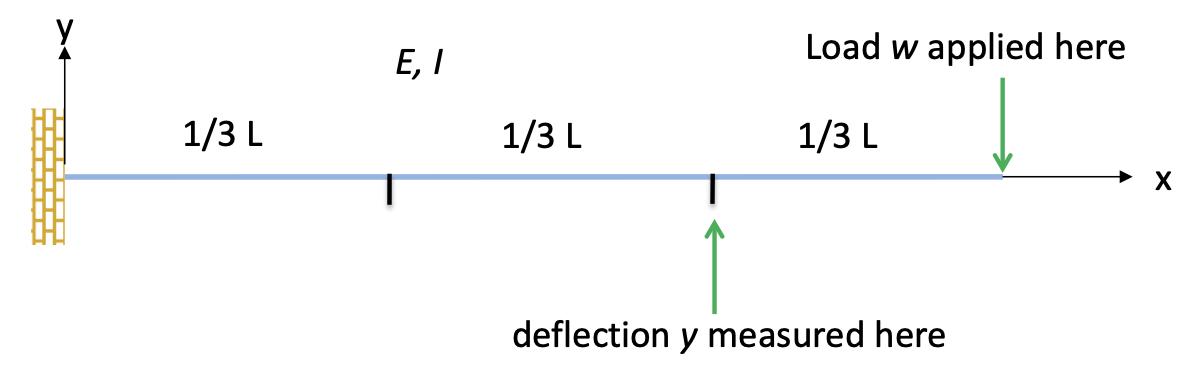
\includegraphics[width=6in]{images/Config 1-3}
\caption{The beam configuration for experiments 1--3.}
\label{fig:config_1-3}
\end{figure}

\begin{figure}[htbp]
\centering
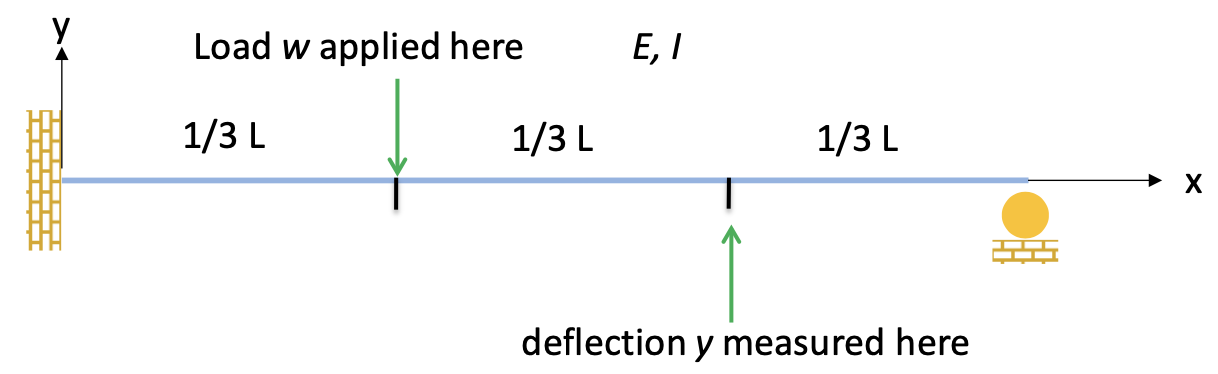
\includegraphics[width=6in]{images/Config 4}
\caption{The beam configuration for experiment 4.}
\label{fig:config_4}
\end{figure}

\begin{figure}[htbp]
\centering
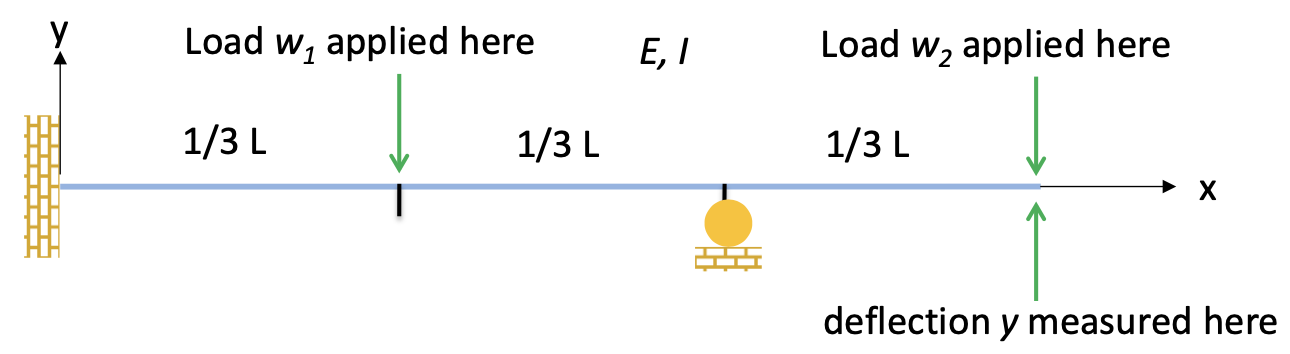
\includegraphics[width=6in]{images/Config 5}
\caption{The beam configuration for experiment 5.}
\label{fig:config_5}
\end{figure}

\section{Procedures} \label{procedures}
% TODO

\section{Data} \label{data}
% TODO

\section{Analysis} \label{analysis}
To derive the following deflection expressions, we are given the following equations of superposition for a cantilever beam:
\begin{align}
	0\le{}x\le{}L_1:y&=-\frac{wx^2}{6EI}(3L_1-x)\label{eqn:superpos_1}\\
	L_1\le{}x\le{}L:y&=-\frac{wL_1^2}{6EI}(3x-L_1)\label{eqn:superpos_2}\\
	L_1=L:y&=-\frac{wx^2}{6EI}(3L-x)\label{eqn:superpos_3}
\end{align}
where $L$ is the length of the beam, $E$ is the elastic modulus of the beam material, $I$ is the beam moment of inertia, $w$ is the applied load, $L_1$ is the distance from the fixed end of the beam to the applied load, and $x$ is the point about which deflection is measured. Note that Equation \ref{eqn:superpos_2} is invalid for $L_1=L$.

The configuration for test four, shown in Figure \ref{fig:config_4}, consists of a beam fixed at one end with a roller support on the other end. A load is being applied at $\frac{1}{3}$ the length, measured from the fixed end. To calculate the deflection at $\frac{2}{3}$ the length, \ie $x=\frac{2}{3}L$, we are given the following equation:
\begin{align} \label{eqn:config_4-deflection}
	\nu&=-\frac{w}{EI}\frac{23}{4374}L^3
\end{align}
where $w$ is the applied load, $E$ is the elastic modulus, $I$ is the moment of inertia, $L$ is the length of the beam, and $\nu$ is the deflection of the beam at $x=\frac{2}{3}L$.

To derive this expression, we first note that the beam configuration is indeterminate. The roller support is redundant and can be replaced by a vertical applied load of magnitude, $R_y$. The beam is now effectively a cantilevered beam with two applied loads. Deflection at a point $x$ can be calculated by summing the deflection at $x$ from each of the applied loads.

The deflection due to the applied load at $x=\frac{1}{3}L$, $\nu_w$, can be derived from Equation \ref{eqn:superpos_2}.
\begin{align*}
	\nu_w(x)&=-\frac{wL_1^2}{6EI}(3x-L_1)\\
	&=-\frac{w\frac{1}{9}L^2}{6EI}(3x-\frac{1}{3}L)\\
	&=-\frac{wL^2}{162EI}(9x-L)
\end{align*}
This expression is true for all $x\in[\frac{1}{3}L,L]$.

The deflection due to the redundant reaction force at $x=L$, $\nu_{R_y}$, can be derived from Equation \ref{eqn:superpos_3}.
\begin{align*}
	\nu_{R_y}(x)&=-\frac{wx^2}{6EI}(3L-x)\\
	&=-\frac{R_yx^2}{6EI}(3L-x)
\end{align*}
This expression is true for all $x\in[0,L]$.

To calculate the deflection at $x=\frac{2}{3}L$, we first need to determine the value of $R_y$. We know from Figure \ref{fig:config_4}, at $x=L$ there is a roller support, and therefore, $\nu(x)=0$ at $x=L$. We apply this boundary condition below to find $R_y$.
\begin{align*}
	\nu(L)&=\nu_w(L)+\nu_{R_y}(L)=0\\
	0&=-\frac{wL^2}{162EI}(9L-L)-\frac{R_yL^2}{6EI}(3L-L)\\
	0&=-\frac{4wL^3}{81EI}-\frac{R_yL^3}{3EI}\\
	R_y&=-\frac{4w}{27}
\end{align*}
Substituting in the derived expression for $R_y$ into the earlier equation for $\nu_{R_y}$, we find that
\begin{align*}
	\nu_{R_y}(x)&=\frac{2wx^2}{81EI}(3L-x)
\end{align*}
Now that we have expressions for both $\nu_w$ and $\nu_{R_y}$ in terms of $w$, we can find the derive an equation for the deflection of the beam at $x=\frac{2}{3}L$ in terms of $w$, $E$, $I$, and $L$.
\begin{align*}
	\nu\left(\frac{2}{3}L\right)&=\nu_w\left(\frac{2}{3}L\right)+\nu_{R_y}\left(\frac{2}{3}L\right)\\
	&=-\frac{wL^2}{162EI}\left(9\left(\frac{2}{3}L\right)-L\right)+\frac{2w\left(\frac{2}{3}L\right)^2}{81EI}\left(3L-\left(\frac{2}{3}L\right)\right)\\
	&=-\frac{5wL^3}{162EI}+\frac{56wL^3}{2187EI}\\
	&=\frac{wL^3}{EI}\left(-\frac{5}{162}+\frac{56}{2187}\right)\\
	&=-\frac{23wL^3}{4374EI}
\end{align*}
As expected, this equation matches the given expression in Equation \ref{eqn:config_4-deflection}. Calculating the theoretical deflection is then trivial. We know $w=(\qty{1000}{\g})(\frac{\qty{1}{\kg}}{\qty{1000}{\g}})(\qty[per-mode=fraction]{9.81}{\m\per\s\squared})=\qty{9.81}{\N}$, $L=\qty{0.90}{\m}$, $E=\qty{68.9e9}{\Pa}$, and $I=\frac{1}{12}(\qty{12.8}{\mm})(\qty{6.4}{\mm})^3(\frac{\qty{1}{\m}}{\qty{1000}{\mm}})^4=\qty{2.796e-10}{\m^4}$. Plugging these values into Equation \ref{eqn:config_4-deflection}, we find that
\begin{align*}
	\nu\left(\frac{2}{3}L\right)&=-\frac{23(\qty{9.81}{\N})(\qty{0.90}{\m})^3}{4374(\qty{68.9e9}{\Pa})(\qty{2.796e-10}{\m^4})}\\
	&=\qty{-1.952}{\mm}\text{ or }\qty{1.952}{\mm}\downarrow
\end{align*}

The configuration for test five, shown in Figure \ref{fig:config_5}, consists of a beam fixed at one end with a roller support at $\frac{2}{3}$ the length. A load is being applied at $\frac{1}{3}$ the length and at the end, measured from the fixed end. To calculate the deflection at the free end of the beam, \ie $x=L$, we are given the following equation:
\begin{align} \label{eqn:config_5-deflection}
	\nu&=-\frac{L^3}{EI}\left(\frac{5w_2}{162}-\frac{w_1}{216}\right)
\end{align}
where $w_1$ is the applied load at $x=\frac{1}{3}L$, $w_2$ is the applied load at $x=L$, $E$ is the elastic modulus, $I$ is the moment of inertia, $L$ is the length of the beam, and $\nu$ is the deflection of the beam at $x=L$.

To derive this expression, we first note that the beam configuration is indeterminate. The roller support is redundant and can be replaced by a vertical applied load of magnitude, $R_y$. The beam is now effectively a cantilevered beam with three applied loads. Deflection at a point $x$ can be calculated by summing the deflection at $x$ from each of the applied loads.

The deflection due to the applied load at $x=\frac{1}{3}$, $\nu_{w_1}$, can be derived from Equation \ref{eqn:superpos_2}.
\begin{align*}
	\nu_{w_1}(x)&=-\frac{wL_1^2}{6EI}(3x-L_1)\\
	&=-\frac{w_1\frac{1}{9}L^2}{6EI}(3x-\frac{1}{3}L)\\
	&=\frac{w_1L^2}{162EI}(9x-L)
\end{align*}
This expression is true for all $x\in[\frac{1}{3}L,L]$.

The deflection due to the redundant reaction force at $x=\frac{2}{3}L$, $\nu_{R_y}$, can be derived from Equation \ref{eqn:superpos_2}.
\begin{align*}
	\nu_{R_y}(x)&=-\frac{wL_1^2}{6EI}(3x-L_1)\\
	&=-\frac{R_y\frac{4}{9}L^2}{6EI}(3x-\frac{2}{3}L)\\
	&=-\frac{2R_yL^2}{81EI}(9x-2L)
\end{align*}
This expression is true for all $x\in[\frac{2}{3}L,L]$.

The deflection due to the applied load at $x=L$, $\nu_{w_2}$, can be derived from Equation \ref{eqn:superpos_3}.
\begin{align*}
	\nu_{w_2}(x)&=-\frac{wx^2}{6EI}(3L-x)\\
	&=-\frac{w_2}x^2{6EI}(3L-x)
\end{align*}
This expression is for all $x\in[0,L]$.

To calculate the deflection at $x=L$, we first need to determine the value of $R_y$. We know from Figure \ref{fig:config_5}), at $x=\frac{2}{3}L$ there is a roller support, and therefore, $\nu(x)=0$ at $x=\frac{2}{3}L$. We apply this boundary condition below to find $R_y$.
\begin{align*}
	\nu(\frac{2}{3}L&=\nu_{w_1}(\frac{2}{3}L)+\nu_{R_y}(\frac{2}{3}L)+\nu_{w_2}(\frac{2}{3}L)=0\\
	0&=-\frac{w_1L^2}{162EI}(9(\frac{2}{3}L)-L)-\frac{2R_yL^2}{81EI}(9(\frac{2}{3}L)-2L)-\frac{w_2\frac{4}{9}L^2}{6EI}(3L-(\frac{2}{3}L)\\
	0&=-\frac{5w_1}{162}-\frac{8R_y}{81}-\frac{14w_2}{81}\\
	R_y&=-\frac{5}{16}(w_1+\frac{28w_2}{5})	
\end{align*}
Now that we have expressions for the deflection due to all the forces, we can derive an equation for the deflection of the beam at $x=L$ using the method of superposition.
\begin{align*}
	\nu(L)&=\nu_{w_1}(L)+\nu_{R_y}(L)+\nu_{w_2}(L)\\
	&=-\frac{w_1L^2}{162EI}(9L-L)-\frac{2\left(-\frac{5}{16}\left[w_1+\frac{28w_2}{5}\right]\right)L^2}{81EI}(9L-2L)-\frac{w_2L^2}{6EI}(3L-L)\\
	&=-\frac{4w_1L^3}{81EI}+\frac{35\left(w_1+\frac{28w_2}{5}\right)L^3}{648EI}-\frac{w_2L^3}{3EI}\\
	&=-\frac{L^3}{EI}\left[\frac{4w_1}{81}-\frac{35w_1}{648}-\frac{49w_2}{162}+\frac{w_2}{3}\right]\\
	&=-\frac{L^3}{EI}\left(\frac{5w_2}{162}-\frac{w_1}{216}\right)
\end{align*}
As expected, this equation matches the given expression in Equation \ref{eqn:config_5-deflection}. Calculating the theoretical deflection is then trivial. We know $w_1=(\qty{2500}{g})(\frac{\qty{1}{kg}}{\qty{1000}{\g}})(\qty[per-mode=fraction]{9.81}{\m\per\s\squared})=\qty{24.53}{\N}$, $w_2=(\qty{200}{\g})(\frac{\qty{1}{\kg}}{\qty{1000}{\g}})(\qty[per-mode=fraction]{9.81}{\m\per\s\squared})=\qty{19.62}{\N}$, $L=\qty{0.90}{\m}$, $E=\qty{68.9e9}{\Pa}$, and $I=\frac{1}{12}(\qty{12.8}{\mm})\cdot(\qty{6.4}{\mm})^3(\frac{\qty{1}{\m}}{\qty{1000}{\mm}})^4=\qty{2.796e-10}{\m^4}$. Plugging these values into Equation \ref{eqn:config_5-deflection}, we find that
\begin{align*}
	\nu(L)&=-\frac{\qty{0.90}{\m}}{(\qty{68.9e9}{\Pa})(\qty{2.796e-10}{\m^4})}\left(\frac{5(\qty{19.62}{\N})}{162}-\frac{\qty{24.53}{\N}}{216}\right)\\
	&=\qty{2.005}{\mm}\text{ or }\qty{2.005}{\mm}\uparrow
\end{align*}

\section{Conclusion} \label{conclusion}
% TODO

\end{document}
